\chapter{Parser}
\label{chap:parser}

\section{Parsebaum}
\label{sec:parsetree}

\subsection{Aufbau}
Der Parsebaum ist ein reiner Binärbaum,
welcher bei Bedarf um Zwischenknoten erweitert wird.
Jeder Knoten hat ein rechtes und ein linkes Kind,
einen Knotentyp, einen Datentyp,
eine Datensektion für Nutzdaten sowie Felder für die Dateikoordinaten des ersten Tokens. \\
Die Interpretation der Inhalte der Datensektion sind Abhängig vom Typ des Knotens.
Enthalten sind ein Feld \texttt{val},
um Integerwerte zu speichern,
ein Feld \texttt{sym} als Zeiger auf ein Element der Symboltabelle
und in \texttt{op} ist der Operator gespeichert.

\begin{lstlisting}
typedef enum {
	OP_NEG,	/* unary - */
	OP_ADD,	/* + */
	OP_SUB,	/* - */
	OP_DIV,	/* / */
	OP_MUL,	/* * */
	OP_LESS,	/* < */
	OP_GRTR,	/* > */
	OP_EQUAL,	/* = */
	OP_UNEQ,	/* <!> */
	OP_NOT,	/* ! (unary) */
	OP_AND	/* & */
} Optype;

typedef struct Node Node;
struct Node {
	Node *left;
	Node *right;
	Nodetype type;
	union {
		vlong  val;
		Symbol *sym;
		Optype op;
	} data;
	uint col;
	uint row;
	Datatype datatype;
};
\end{lstlisting}

\subsection{Knotentypen}

\begin{lstlisting}
typedef enum {
	NODE_NONE,
	/* nonterminal symbols */
	NODE_PROG,
	NODE_DECLS,
	NODE_DECL,
	NODE_ARRAY,
	NODE_STATEMENTS,
	NODE_STATEMENT,
	NODE_EXP,
	NODE_EXP2,
	NODE_INDEX,
	NODE_OPEXP,
	NODE_OP,
	/* terminal symbols */
	NODE_PRINT,
	NODE_READ,
	NODE_IF,
	NODE_WHILE,
	NODE_IDENT,
	NODE_INTCONST
} Nodetype;
\end{lstlisting}

\subsubsection{Leerer Knoten \texttt{NODE\_NONE}}
\label{sec:nonenode}
Dieser Knotentyp beschreib einen Knoten ohne semantische Bedeutung.
Daher wird er als Zwischenknoten eingesetzt,
wenn ein Knotentyp mehr als zwei Kindknoten benötigt.
Da er in der Enumeration den Wert \texttt{0} annimmt ist er außerdem der Standardtyp für Knoten,
bei welchen kein anderer Typ gesetzt wurde.

\subsubsection{Wurzelknoten \texttt{NODE\_PROG}}
\label{sec:prognode}
\texttt{left} enthält die Liste aller Deklarationen,
\texttt{right} die Liste aller Ausdrücke.
Daher wird von den übrigen Programmteilen erwartet,
dass es sich beim linken Kindknoten um einen \hyperref[sec:declsnode]{Deklarationslistenknoten} und beim rechten Kindknoten um einen \hyperref[sec:stmtsnode]{Anweisungslistenknoten} handelt.

Eine schematische Darstellung findet sich in \hyperref[fig:prognode]{Abbildung~\ref{fig:prognode}}.

\begin{figure}[h!]
\centering
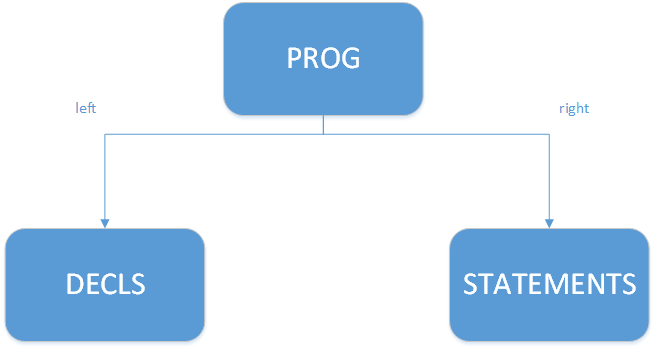
\includegraphics[width=0.7\linewidth]{PROG}
\caption{\texttt{PROG}-Knoten}
\label{fig:prognode}
\end{figure}

\subsubsection{Deklarationslistenknoten \texttt{NODE\_DECLS}}
\label{sec:declsnode}
Deklarationslistenknoten enthalten als linkes Kind einen \hyperref[sec:declnode]{Deklarationsknoten} und rechts einen weiteren Deklarationslistenknoten.
Wenn kein weiterer Listenknoten folgt,
dann ist der Zeiger \texttt{NULL}.

Eine schematische Darstellung findet sich in \hyperref[fig:declsnode]{Abbildung~\ref{fig:declsnode}}.

\begin{figure}[h!]
\centering
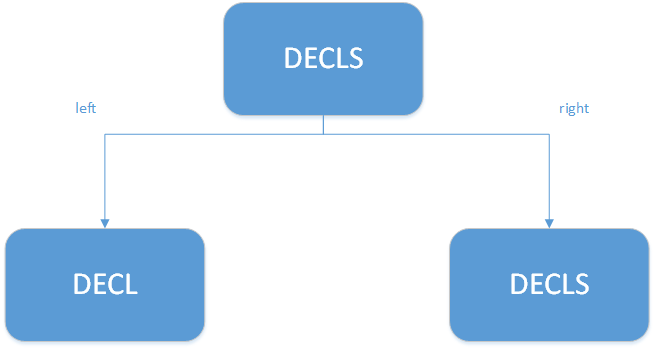
\includegraphics[width=0.7\linewidth]{DECLS}
\caption{\texttt{DECLS}-Knoten}
\label{fig:declsnode}
\end{figure}

\subsubsection{Deklarationsknoten \texttt{NODE\_DECL}}
\label{sec:declnode}
Ein Deklarationsknoten enthält in \texttt{data.sym} einen Zeiger auf ein Element der Symboltabelle.
Wenn es sich bei der deklarierten Variable um ein Array handelt,
dann zeit \texttt{left} auf einen \hyperref[sec:arraynode]{Arrayknoten},
ansonsten sind beide Kinder \texttt{NULL}.

Eine schematische Darstellung mitsamt einem \hyperref[sec:arraynode]{Arrayknoten} findet sich in \hyperref[fig:declnode]{Abbildung~\ref{fig:declnode}}.

\begin{figure}[h!]
\centering
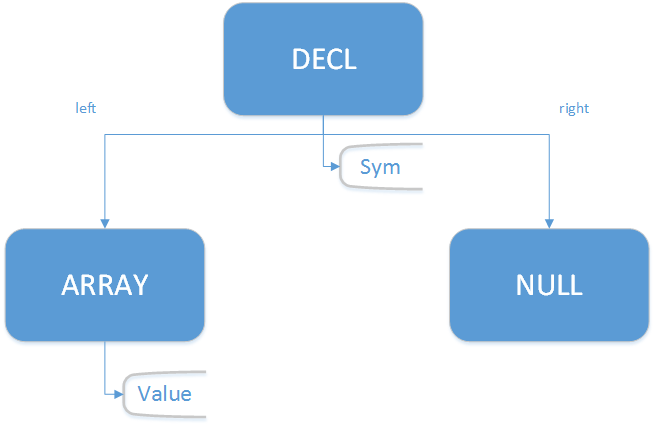
\includegraphics[width=0.7\linewidth]{DECL_ARRAY}
\caption{\texttt{DECL}-Knoten mit einem angeschlossenen \texttt{ARRAY}-Knoten}
\label{fig:declnode}
\end{figure}

\subsubsection{Arrayknoten \texttt{NODE\_ARRAY}}
\label{sec:arraynode}
Ein Arrayknoten enthält lediglich die Deklarationsgröße in \texttt{data.val}.

Die schematische Darstellung ist mit in \hyperref[fig:declnode]{Abbildung~\ref{fig:declnode}} enthalten.

\subsubsection{Anweisungslistenknoten \texttt{NODE\_STATEMENTS}}
\label{sec:stmtsnode}
Ein Anweisungslistenknoten gleicht im Aufbau einem \hyperref[sec:declsnode]{Deklarationslistenknoten},
mit dem Unterschied dass \texttt{left} immer auf einen \hyperref[sec:stmtnode]{Anweisungsknoten} zeigt.
Im Sonderfall der \texttt{\{\ldots\}}-Anweisung sind aber beide Zeiger \texttt{NULL}.

Eine schematische Darstellung steht in \hyperref[fig:stmtsnode]{Abbildung~\ref{fig:stmtsnode}} zur Verfügung.

\begin{figure}[h!]
\centering
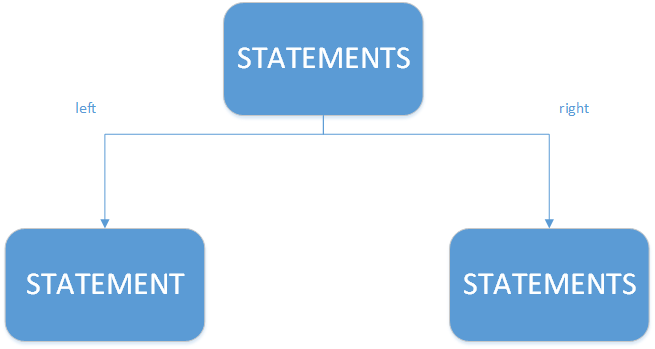
\includegraphics[width=0.7\linewidth]{STATEMENTS}
\caption{\texttt{STATEMENTS}-Knoten}
\label{fig:stmtsnode}
\end{figure}

\subsubsection{Anweisungsknoten \texttt{NODE\_STATEMENT}}
\label{sec:stmt}
Ein Anweisungsknoten verfügt immer über verschiedene Unterknoten im linken Teilbaum:

\begin{itemize}
\item \texttt{NODE\_IDENT}

Ein Zuweisungsknoten enthält in seinem Datensegment einen Zeiger auf ein Symbol in der Symboltabelle.
Der rechte Teilbaum des Anweisungsknotens enthält in diesem Fall zunächst einen \hyperref[sec:nonenode]{leeren Knoten},
welcher mit \texttt{left} wiederrum auf einen \hyperref[sec:indexnode]{Indexknoten} und mit \texttt{right} auf einen \hyperref[sec:expnode]{Ausdrucksknoten} zeigt.
Der Indexknoten kann auch \texttt{NULL} sein,
wenn es sich bei der durch \texttt{NODE\_IDENT->data.sym} beschriebenen Variable nicht um ein Array handelt.

Eine schematische Darstellung findet sich in \hyperref[fig:assgin]{Abbildung~\ref{fig:assgin}}.

\item \texttt{NODE\_PRINT}

Ein Ausgabeknoten enthält den auszugebenden \hyperref[sec:expnode]{Ausdruck} in \texttt{left}.

Eine schematische Darstellung findet sich in \hyperref[fig:print]{Abbildung~\ref{fig:print}}.

\item \texttt{NODE\_READ}

Ein Eingabeknoten enthält in \texttt{left} einen Variablenknoten,
in welchem die Eingabe gespeichert wird.
Da es sich bei der Variable um ein Array handeln kann,
befindet sich in \texttt{right} eventuell ein \hyperref[sec:indexnode]{Indexknoten}.

Eine schematische Darstellung findet sich in \hyperref[fig:read]{Abbildung~\ref{fig:read}}.
\item \texttt{NODE\_STATEMENTS}

Da geschweifte Klammern lediglich der Gruppierung von Anweisungen dienen,
werden sie im Parsebaum lediglich durch einen \hyperref[sec:stmtsnode]{Anweisungslistenknoten} repräsentiert.
Da im \hyperref[sec:typecheck]{Typchecker} direkt der linke Kindknoten eines Anweisungsknotens überprüft wird,
ergibt sich hieraus der beim Anweisungslistenknoten beschriebene Sonderfall.

Eine schematische Darstellung findet sich in \hyperref[fig:stmts]{Abbildung~\ref{fig:stmts}}.

\item \texttt{NODE\_IF}

Wenn in \texttt{left}-Feld eines Anweisungsknotens ein Verzweigungsknoten auftritt,
dann zeigt \texttt{right} auf einen \hyperref[sec:expnode]{Ausdrucksknoten}.
Beide Kindknoten des Verzweigungsknotens beinhalten weitere Anweisungsknoten,
wobei in \texttt{left} die \texttt{if}-Verzweigung gespeichert ist und in \texttt{right} die \texttt{else}-Verzweigung.

Eine schematische Darstellung findet sich in \hyperref[fig:if]{Abbildung~\ref{fig:if}}.

\item \texttt{NODE\_WHILE}

Ein Schleifenknoten in \texttt{left} den Rumpfausdruck,
wobei es sich um einen weiteren Anweisungsknoten handelt.
Die Schleifenbedingung wird im \texttt{right}-Feld des Anweisungsknoten,welcher die Wiederholungsanweisung entält gespeichert,
wobei es sich um einen \hyperref[sec:expnode]{Ausdrucksknoten} handelt.

Eine schematische Darstellung findet sich in \hyperref[fig:while]{Abbildung~\ref{fig:while}}.

\end{itemize}

\begin{figure}[h!]
\centering
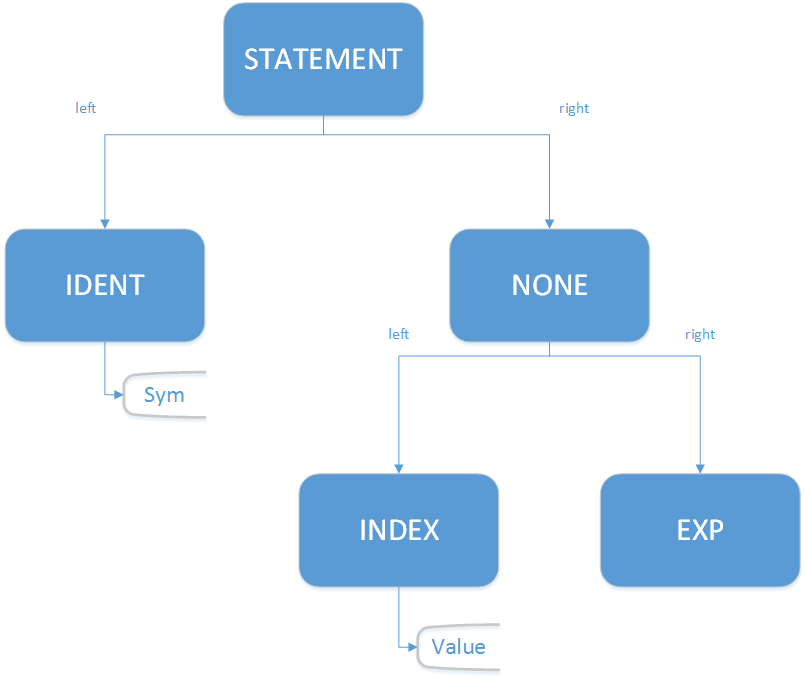
\includegraphics[width=\linewidth]{STMT_ASSIGN}
\caption{\texttt{STATEMENT}-Knoten mit einer Zuweisung}
\label{fig:assgin}
\end{figure}

\begin{figure}[h!]
\centering
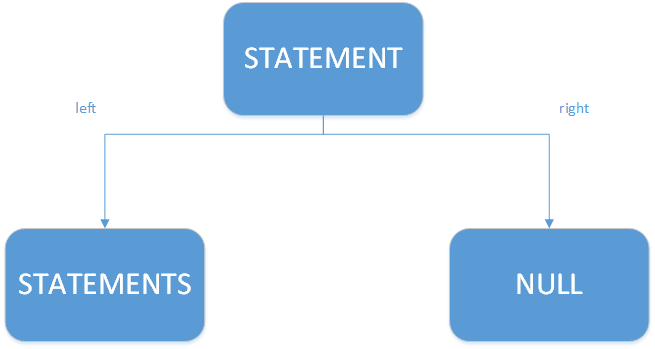
\includegraphics[width=0.7\linewidth]{STMT_STMTS}
\caption{\texttt{STATEMENT}-Knoten mit einem Anweisungsblock}
\label{fig:stmts}
\end{figure}

\begin{figure}[h!]
\centering
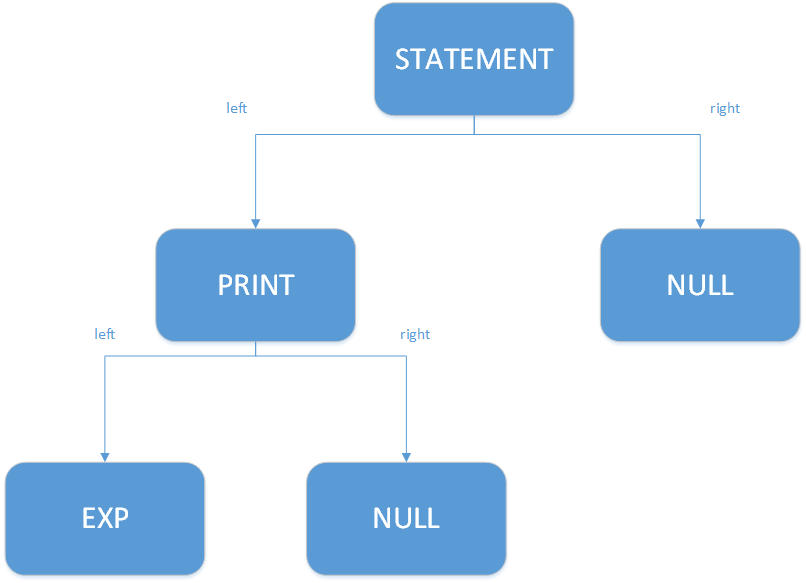
\includegraphics[width=\linewidth]{STMT_PRINT}
\caption{\texttt{STATEMENT}-Knoten mit Ausgabeanweisung}
\label{fig:print}
\end{figure}

\begin{figure}[h!]
\centering
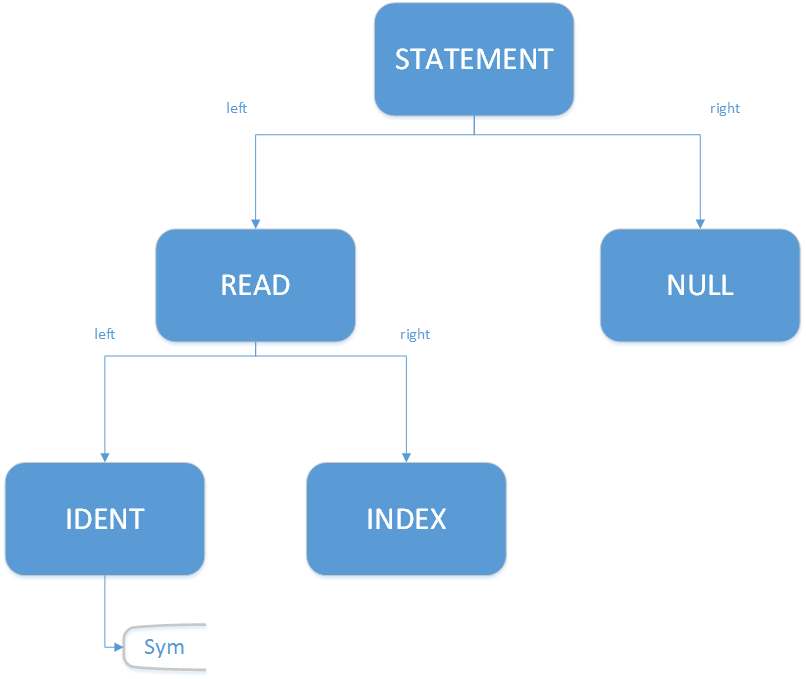
\includegraphics[width=\linewidth]{STMT_READ}
\caption{\texttt{STATEMENT}-Knoten mit Eingabeanweisung}
\label{fig:read}
\end{figure}

\begin{figure}[h!]
\centering
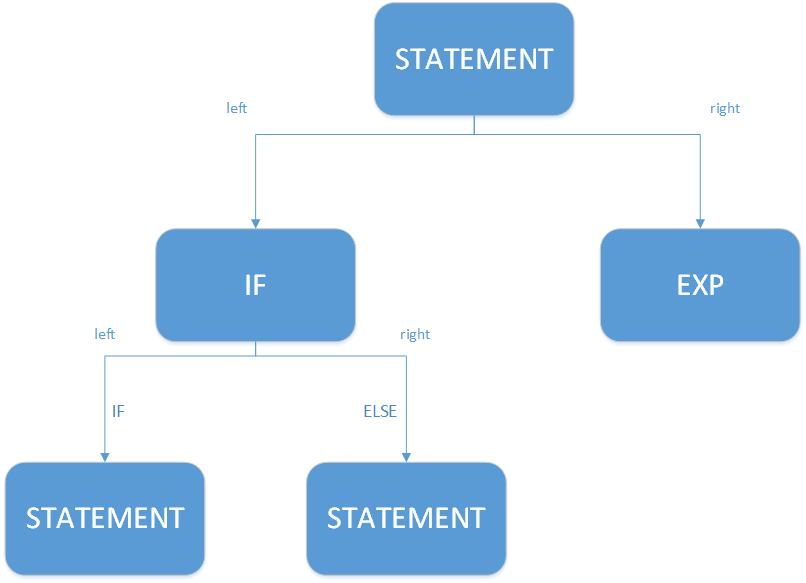
\includegraphics[width=\linewidth]{STMT_IF}
\caption{\texttt{STATEMENT}-Knoten mit Verzweigungsanweisung}
\label{fig:if}
\end{figure}

\begin{figure}[h!]
\centering
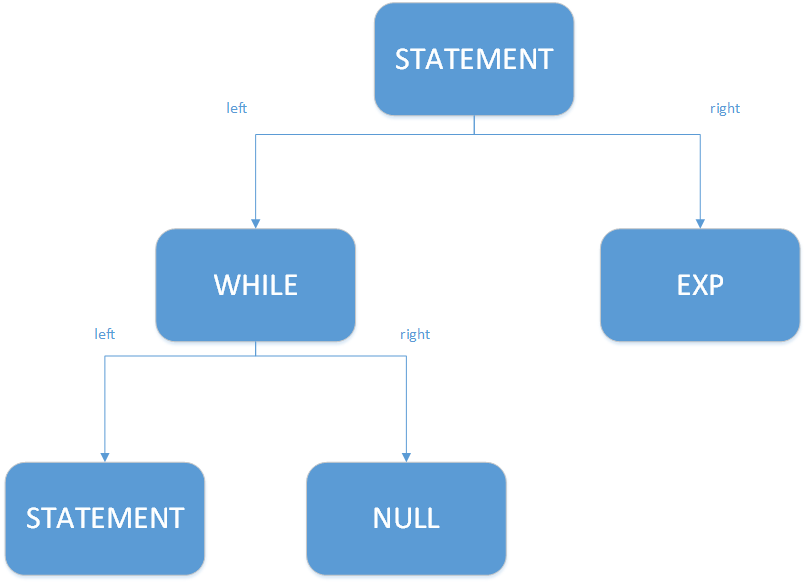
\includegraphics[width=\linewidth]{STMT_WHILE}
\caption{\texttt{STATEMENT}-Knoten mit Schleifenanweisung}
\label{fig:while}
\end{figure}

\subsubsection{Ausdrucksknoten \texttt{NODE\_EXP}}
\label{sec:expnode}
Ein Ausdrucksknoten zeigt mit \texttt{left} auf einen \hyperref[sec:exp2node]{Teilausdrucksknoten} und mit \texttt{right} auf einen \hyperref[sec:opexpnode]{Operatorausdrucksknoten}.
Dieser kann \texttt{NULL} sein, wenn kein Operatorausdruck vorliegt.

Eine schematische Darstellung findet sich in \hyperref[fig:expnode]{Abbildung~\ref{fig:expnode}}.

\begin{figure}[h!]
\centering
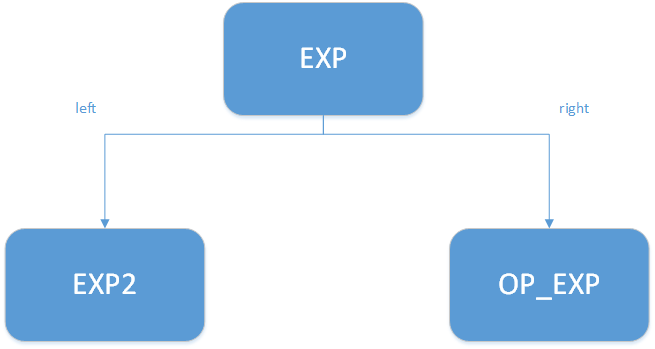
\includegraphics[width=0.7\linewidth]{EXP}
\caption{\texttt{EXP}-Knoten}
\label{fig:expnode}
\end{figure}

\subsubsection{Teilausdrucksknoten \texttt{NODE\_EXP2}}
\label{sec:exp2node}
Ein Teilausdrucksknoten wird anhand des linken Kindknotens weiter differenziert.

\begin{itemize}
\item \texttt{NODE\_EXP}

Ein geklammerter Ausdruck wird durch einen einzelnen \hyperref[sec:expnode]{Ausdrucksknoten} im linken Teilbaum dargestellt.

Eine schematische Darstellung findet sich in \hyperref[fig:exp]{Abbildung~\ref{fig:exp}}.

\item \texttt{NODE\_IDENT}

Eine Variable wird durch einen Knoten vom Typ \texttt{NODE\_IDENT} symbolisiert.
Falls es sich bei der Variable um ein Array handelt,
hat der Teilausdrucksknoten einen \hyperref[sec:indexnode]{Indexknoten} im rechten Teilbaum.

Eine schematische Darstellung findet sich in \hyperref[fig:ident]{Abbildung~\ref{fig:ident}}.

\item \texttt{NODE\_INTCONST}

Ein Integer enthält im Datensegment den Wert im Feld \texttt{data.val}.

Eine schematische Darstellung findet sich in \hyperref[fig:intconst]{Abbildung~\ref{fig:intconst}}.

\item \texttt{NODE\_OP}

Unäre Operatoren setzen sich aus einem \hyperref[sec:opnode]{Operatorknoten} im linken Kind des Teilausdruckknotens sowie einem weiteren Teilausdruck im linken Unterbaum zusammen.

Eine schematische Darstellung findet sich in \hyperref[fig:op]{Abbildung~\ref{fig:op}}.

\end{itemize}

\begin{figure}[h!]
\centering
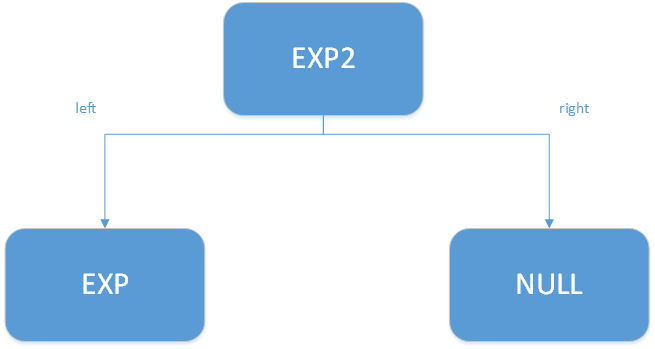
\includegraphics[width=0.7\linewidth]{EXP2_EXP}
\caption{\texttt{EXP2}-Knoten mit geklammertem Ausdruck}
\label{fig:exp}
\end{figure}

\begin{figure}[h!]
\centering
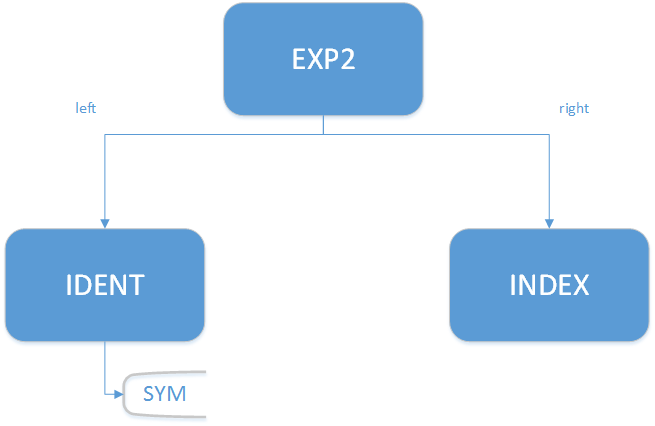
\includegraphics[width=0.7\linewidth]{EXP2_IDENT}
\caption{\texttt{EXP2}-Knoten mit Variable}
\label{fig:ident}
\end{figure}

\begin{figure}[h!]
\centering
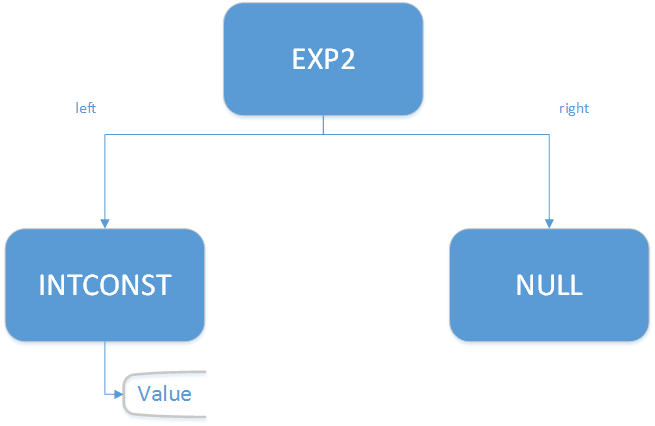
\includegraphics[width=0.7\linewidth]{EXP2_INTCONST}
\caption{\texttt{EXP2}-Knoten mit Integer-Konstante}
\label{fig:intconst}
\end{figure}

\begin{figure}[h!]
\centering
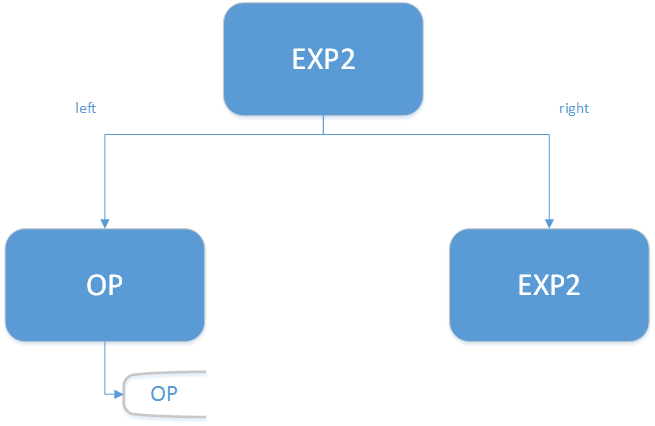
\includegraphics[width=0.7\linewidth]{EXP2_OP}
\caption{\texttt{EXP2}-Knoten mit unärem Operator}
\label{fig:op}
\end{figure}

\subsubsection{Indexknoten \texttt{NODE\_INDEX}}
\label{sec:indexnode}
Ein Indexknoten verfügt nur über ein einzelnen Kindknoten,
welches in \texttt{left} gespeichert ist.
Dabei handelt es sich um einen \hyperref[sec:expnode]{Ausdrucksknoten}.

Eine schematische Darstellung findet sich in \hyperref[fig:indexnode]{Abbildung~\ref{fig:indexnode}}.

\begin{figure}[h!]
\centering
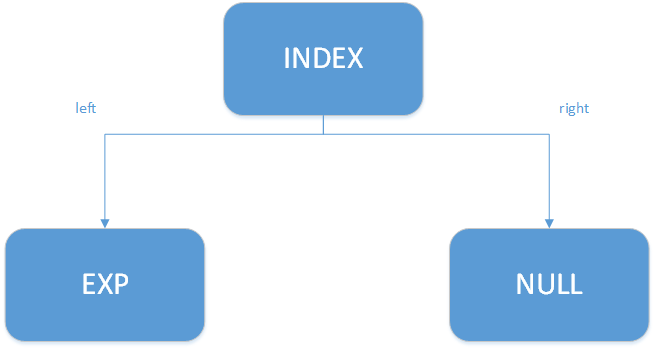
\includegraphics[width=0.7\linewidth]{INDEX}
\caption{\texttt{INDEX}-Knoten}
\label{fig:indexnode}
\end{figure}

\subsubsection{Operatorausdrucksknoten \texttt{NODE\_OPEXP}}
\label{sec:opexpnode}
Die Kindknoten eines Operatorausdrucksknotens sind links ein \hyperref[sec:opnode]{Operatorknoten} und rechts ein \hyperref[sec:expnode]{Ausdrucksknoten}.
Er enthält keine weiteren Daten.

Eine schematische Darstellung findet sich in \hyperref[fig:opexpnode]{Abbildung~\ref{fig:opexpnode}}.

\begin{figure}[h!]
\centering
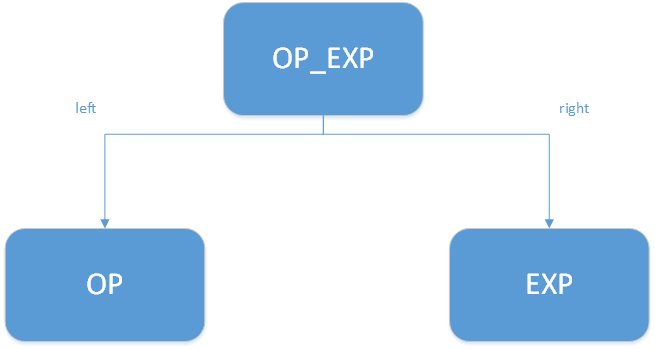
\includegraphics[width=0.7\linewidth]{OP_EXP}
\caption{\texttt{OP\_EXP}-Knoten}
\label{fig:opexpnode}
\end{figure}

\subsubsection{Operatorknoden \texttt{NODE\_OP}}
\label{sec:opnode}
Ein Operatorknoten enthält lediglich einen Operator in \texttt{data.op}.

Eine schematische Darstellung findet sich in \hyperref[fig:opnode]{Abbildung~\ref{fig:opnode}}.

\begin{figure}[h!]
\centering
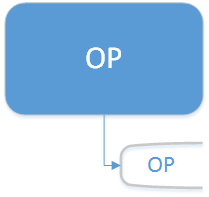
\includegraphics{OP}
\caption{\texttt{OP}-Knoten}
\label{fig:opnode}
\end{figure}

\subsection{Funktionen}

Für den Parsebaum steht nur eine einzige Funktion zur Verfügung,
welche einen Konstruktor für die einzelnen Knoten repräsentiert.
Diese Funktion ist zusammen mit einem durch den \texttt{Nodetype} indizierbaren String-Array für die Knotennamen in der Datei \texttt{btree.c} definiert.

\begin{lstlisting}
Node *makenode(Nodetype type, uint row, uint col);
\end{lstlisting}

Als Argumente akzeptiert sie den Knotentyp sowie die Zeile und Spalte des ersten Tokens,
welche durch den Knoten repräsentiert werden.

\clearpage

\section{Parser}

\subsection{Übersicht}
Bei diesem Parser handelt sich es um einen linksrekursiv absteigenden Parser.
Er stellt nur eine einzige Funktion öffentlich zur Verfügung:

\begin{lstlisting}
void parseprog(void);
\end{lstlisting}

Diese Routine legt den Wurzelknoten \texttt{NODE\_PROG} neu an und speichert diesen in der Variable \texttt{parsetree},
welche eine globale Variable des Compilerprogrammes ist.
Dann wird das erste Token vom Scanner angefordert,
damit dies in der nichtöffentlichen Variable \texttt{nexttoken} zur Verfügung steht.
Dadurch kann diese zum Vorrausschauen auf das nächste Symbol verwendet werden.
Dann werden der linke und der rechte Teilbaum mit den für die Knoten passenden Prozeduren aufgebaut.
Jeder Knoten, welcher einem Nichtterminalsymbol der Sprache spricht,
hat eine entsprechende \texttt{parse\ldots}-Funktion,
welche wiederrum ihre Teilbäume aufbaut.

Wenn eine dieser Funktionen Tokens konsumieren möchte,
dann ruft sie dazu die statische Funktion \texttt{match} auf,
welche ein \texttt{Symboltype} als Argmument nimmt.
Wenn der Symboltyp des nächsten Tokens mit diesem übereinstimmt,
dann wird ein neues Token angefordert.
Daher werden Operationen wie beispielsweise das Auslesen des Symbols der Symboltabelle von Variablen vor dem Aufruf von \texttt{match()} durchgeführt,
da diese Informationen danach verloren sind.

Die Vorrausschau wird auch bei Nichtterminalen eingesetzt,
welche zu ε expandieren.
Wenn das Lookahead-Symbol nicht passt,
wird der Zeiger auf den entsprechenden Kindknoten auf \texttt{NULL} belassen.
Für \texttt{STATEMENT} und \texttt{OP\_EXP} sind diese Mengen jedoch relativ umfangreich,
weshalb für diesen Zweck die Macros \texttt{FIRST\_STATEMENT} und \texttt{FIRST\_OP\_EXP} zum Einsatz kommen.
Diese expandieren lediglich zu einem Wahrheitswert,
welcher die Verfügbarkeit eines passenden Tokens repräsentiert.

Die übrigen Funktionen stellen lediglich den in \hyperref[sec:parsetree]{Abschnitt~\ref{sec:parsetree}} zusammen,
weshalb die dortige Dokumentation als ausreichend eingeschätzt wird.
